% Paper 1: The Deployment Gap
%
% =============================================================================
% STATUS: PUBLICATION READY
% Last updated: 2026-02-04
% =============================================================================
%
% 13 models evaluated (8 vendors, 4 countries), 29,900 total predictions
% 5 task types: T1 (CLINC), T2 (HotpotQA), T3 (Tools), T4 (BFCL), T5 (SWE)
% Key finding: Spearman rho = +0.09 (p = 0.76) at 2s SLO — accuracy does not
% predict deployment success.
% =============================================================================
\documentclass[11pt]{article}

\usepackage[margin=1in]{geometry}
\usepackage{amsmath,amssymb}
\usepackage{booktabs}
\usepackage{tabularx}
\usepackage{graphicx}
\usepackage{adjustbox}
\usepackage{xcolor}
\usepackage{enumitem}
\usepackage{listings}
\usepackage{tikz}
\usetikzlibrary{arrows.meta, positioning, shapes.geometric, calc}
\usepackage{pgfplots}
\pgfplotsset{compat=1.17}

\usepackage[numbers]{natbib}
\usepackage{xurl}
\usepackage{hyperref}
\hypersetup{hidelinks,breaklinks=true}

\newcommand{\pninetyfive}{\ensuremath{\mathrm{p95}}}
\newcommand{\pninetynine}{\ensuremath{\mathrm{p99}}}
\newcommand{\slo}{\ensuremath{\mathrm{SLO}}}

\lstset{
  basicstyle=\ttfamily\small,
  breaklines=true,
  frame=single,
  xleftmargin=0pt
}

\title{The Deployment Gap: Why Benchmark Accuracy\\Fails to Predict Production Readiness}

\author{
V. Michael Maloney \\
Neuralift; University of New Hampshire \\
\texttt{mike@neuralift.ai}
}

\date{}

\usepackage{fancyhdr}
\pagestyle{fancy}
\fancyhf{}
\renewcommand{\headrulewidth}{0pt}
\cfoot{\thepage}

\begin{document}
\maketitle
\begin{center}
\textit{Preprint. Work in progress.}
\end{center}

\begin{abstract}
Model selection for production deployment relies heavily on accuracy benchmarks, yet these benchmarks measure only one dimension of readiness. We investigate whether accuracy rankings predict deployment success when latency constraints are imposed.

We evaluate 13 models on five structured output tasks---intent classification, grounded QA, tool calling, function routing, and code patching---under a 2-second latency deadline. What we found was stark: of 29,900 evaluation requests across all models, only 9.3\% from the smallest model arrived both correct and on time. Every other model---all twelve of them---failed to deliver a single request within the deadline.

\begin{center}
\begin{tabular}{llcc}
\toprule
\textbf{Model} & \textbf{Vendor} & \textbf{JSON Valid} & \textbf{Success@SLO} \\
\midrule
Llama-3.2-1B & Meta & 100.0\% & \textbf{9.3\%} (best) \\
Llama-3.2-3B & Meta & 99.9\% & 0.0\% \\
Qwen2.5-3B & Alibaba & 99.7\% & 0.0\% \\
Phi-3-mini & Microsoft & 99.2\% & 0.0\% \\
Qwen3-4B & Alibaba & 99.9\% & 0.0\% \\
Yi-1.5-6B & 01.AI & 99.2\% & 0.0\% \\
Mistral-7B-v0.3 & Mistral & 99.7\% & 0.0\% \\
Falcon-Mamba-7B & TII & 99.8\% & 0.0\% \\
Ministral-8B & Mistral & 99.7\% & 0.0\% \\
Llama-3.1-8B & Meta & 99.8\% & 0.0\% \\
Gemma-2-9B & Google & 99.7\% & 0.0\% \\
Gemma-3-12B & Google & 99.6\% & 0.0\% \\
GPT-OSS-20B & OpenAI & 99.1\% & 0.0\% (worst) \\
\bottomrule
\end{tabular}
\end{center}

The deployment gap---the difference between accuracy and Success@SLO---exceeds 90\% for every model we tested. Twelve of thirteen models achieve near-perfect accuracy while delivering zero production value under realistic latency constraints.

We swept deadline thresholds from 2s to 10s. At production-realistic deadlines, accuracy has no predictive power for deployment success (Spearman $\rho = 0.09$ at 2s). Even at a generous 10-second deadline, 10 of 13 models change rank between accuracy and Success@SLO orderings. This is not an artifact of aggressive thresholds---the disconnect persists regardless of where the line is drawn.

The pattern holds across vendors and architectures: Meta, Alibaba, Microsoft, Google, OpenAI, Mistral, 01.AI, and TII models from the US, China, France, and UAE all show the same inversion. Bigger models that dominate accuracy leaderboards collapse under latency constraints.

We introduce \emph{Success@SLO}---the fraction of requests that are both correct AND arrive on time. This single metric captures what production systems actually experience. We also release SpecSLOEval, a framework for measuring structure, accuracy, faithfulness, stability, and latency across five task types through a unified evaluation harness.

Accuracy-only evaluation is insufficient for deployment decisions.
\end{abstract}

%==============================================================================
\section{Introduction}
%==============================================================================

Most teams pick their production model the same way: find the highest-scoring option on MMLU or HELM that fits the memory budget, integrate it, and ship. It seems reasonable. Better accuracy should mean better results, right?

We tested this assumption with 13 models across five task types and 2,300 structured output examples per model. The results reveal a systematic pattern.

Every model we tested achieves near-perfect accuracy---99\% or higher on producing valid JSON responses. Under a 2-second latency deadline, twelve of those thirteen models deliver exactly zero successful requests. Not low success rates. Zero. The only exception is Llama-3.2-1B, the smallest model in our study, which manages 9.3\% Success@SLO. The deployment gap isn't a few percentage points. It's the difference between ``works in the lab'' and ``works in production.''

Consider what this means in practice. Gemma-3-12B achieves 99.6\% JSON validity and 72.4\% task accuracy, and excels at tool calling (66.5\% success). Its median latency is 40 seconds. GPT-OSS-20B, OpenAI's first open-weights model, hits 99.1\% accuracy with strong function routing (58.2\%). Its P95 latency is 73 seconds. These models aren't failing because they're bad at their jobs. They're failing because production doesn't wait.

We call this the \textbf{deployment gap}---the chasm between what benchmarks promise and what production delivers. Traditional evaluations ask: ``Can this model produce correct answers?'' Production asks a different question entirely: ``Will this model produce correct answers before my users give up?'' Our data suggests these questions have opposite answers. The models that excel at accuracy are precisely the ones that fail at deployment.

The consequences are practical. An engineering team evaluates models on MMLU, selects the accuracy leader, invests weeks in integration, and deploys with confidence---only to find that the majority of production requests exceed the latency SLA. The subsequent rollback reveals what the benchmarks never measured: whether the model could meet a basic latency target under realistic serving conditions.

\begin{figure}[t]
\centering
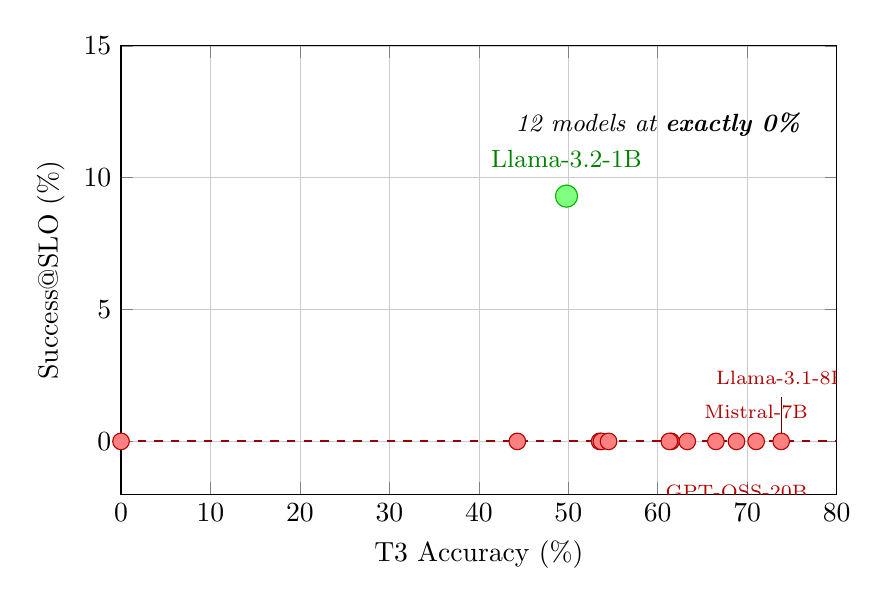
\begin{tikzpicture}
\begin{axis}[
    width=0.88\linewidth,
    height=0.6\linewidth,
    xlabel={T3 Accuracy (\%)},
    ylabel={Success@SLO (\%)},
    xmin=0, xmax=80,
    ymin=-2, ymax=15,
    grid=both,
    grid style={line width=0.1pt, draw=gray!20},
    major grid style={line width=0.2pt, draw=gray!40},
    scatter/classes={
        winner={mark=*,draw=green!70!black,fill=green!50,mark size=4pt},
        loser={mark=*,draw=red!70!black,fill=red!50,mark size=3pt}
    },
]
% Only Llama-3.2-1B survives; all others at 0%
\addplot[scatter, only marks, scatter src=explicit symbolic] coordinates {
    (49.8, 9.3) [winner]
    (53.5, 0.0) [loser]
    (61.5, 0.0) [loser]
    (63.3, 0.0) [loser]
    (61.3, 0.0) [loser]
    (44.3, 0.0) [loser]
    (71.0, 0.0) [loser]
    (0.0, 0.0) [loser]
    (53.7, 0.0) [loser]
    (73.8, 0.0) [loser]
    (54.5, 0.0) [loser]
    (66.5, 0.0) [loser]
    (68.8, 0.0) [loser]
};
\node[anchor=south, font=\small, text=green!50!black] at (axis cs:49.8,10) {Llama-3.2-1B};
\node[anchor=south, font=\scriptsize, text=red!70!black] at (axis cs:73.8,1.8) {Llama-3.1-8B};
\draw[thin, red!40!black] (axis cs:73.8,0.2) -- (axis cs:73.8,1.7);
\node[anchor=south, font=\scriptsize, text=red!70!black] at (axis cs:71.0,0.5) {Mistral-7B};
\node[anchor=north, font=\scriptsize, text=red!70!black] at (axis cs:68.8,-1.3) {GPT-OSS-20B};
% Horizontal line at y=0 to emphasize the cliff
\addplot[dashed, thick, red!60!black] coordinates {(0, 0) (80, 0)};
\node[align=center, font=\small\itshape] at (axis cs:60,12) {12 models at \textbf{exactly 0\%}};
\end{axis}
\end{tikzpicture}
\caption{\textbf{The Deployment Gap.} Accuracy vs Success@SLO for 13 models under a 2-second SLO. This isn't a correlation---it's a cliff. Twelve of thirteen models achieve \textbf{exactly 0\% Success@SLO}, regardless of accuracy. The highest-accuracy model (Llama-3.1-8B, 73.8\%) delivers zero value in production. Only the smallest model (Llama-3.2-1B, 49.8\% accuracy) survives at 9.3\%.}
\label{fig:deployment-gap}
\end{figure}

We focus specifically on single-GPU deployments because this is the \emph{dominant} deployment mode for open-weight models.
Not everyone has a fleet of A100s---and most organizations never will.
Industry surveys and NVIDIA's own guidance~\citep{nvidia2025slm} indicate that the majority of on-premise LLM deployments use 1--2 consumer GPUs behind LM Studio, Ollama, or similar serving stacks, partly for cost, partly to keep sensitive data on-premise.
These setups face all the same production pressures as cloud deployments---schema contracts, faithfulness requirements, latency SLOs---but with tighter resource envelopes and more visible tail behavior.
By evaluating on the hardware where practitioners actually deploy, our results reflect the deployment reality rather than a cluster-based aspiration.

The research community has attacked pieces of this problem.
Serving systems like vLLM~\citep{kwon2023vllm} and SGLang~\citep{zheng2023sglang} optimize throughput and tail latency, but treat the model as a black box emitting unconstrained text.
Structured output tools~\citep{geng2025jsonschemabench,openaiStructuredOutputs} improve syntactic validity, but evaluation stops at ``does it parse?''
What nobody has built is a framework that measures the full stack: structure \emph{and} accuracy \emph{and} faithfulness \emph{and} stability \emph{and} latency, all evaluated together against explicit contracts and deadlines.

\paragraph{What we contribute.}
Three things, in order of how much they will change your workflow:

\begin{enumerate}[leftmargin=12pt]
    \item \textbf{A spec compiler that actually works across backends.}
    Hand us a JSON Schema; we will turn it into whatever your serving stack can enforce, then validate the output anyway because we do not trust the enforcement to be complete.
    If validation fails, we retry with bounded budget.
    All of this gets reflected in your latency measurements, because pretending retries are free is how you end up surprised in production.

    \item \textbf{Success@SLO as your deployment metric.}
    We define this as the fraction of requests that pass your quality gates \emph{and} finish before your deadline.
    Not accuracy alone.
    Not latency alone.
    The joint distribution, because that is what your users experience.

    \item \textbf{Honest measurements from a single GPU.}
    We ran the full configuration ladder---unconstrained, provider-structured, validation-and-retry, grammar-constrained, self-consistency---on real hardware you can buy for under \$4,000.
    No cluster, no cloud dependency, no hidden inference costs.
    The results are uncomfortable but reproducible.
\end{enumerate}


\begin{figure}[t]
\centering
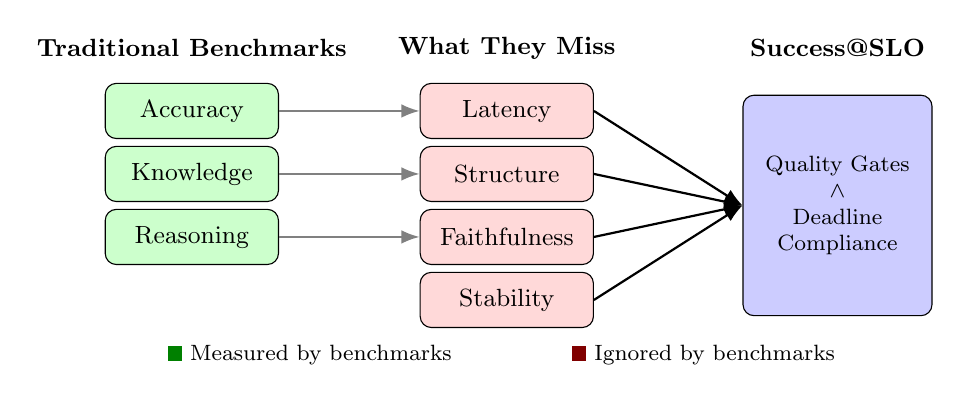
\begin{tikzpicture}[
    font=\small,
    box/.style={draw, rounded corners, minimum width=2.2cm, minimum height=0.7cm, align=center},
    measured/.style={box, fill=green!20},
    missed/.style={box, fill=red!15},
    arrow/.style={-Latex, thick}
]
% Traditional benchmarks column
\node[font=\small\bfseries] at (-4, 3.2) {Traditional Benchmarks};
\node[measured] (acc) at (-4, 2.4) {Accuracy};
\node[measured] (know) at (-4, 1.6) {Knowledge};
\node[measured] (reason) at (-4, 0.8) {Reasoning};

% What they miss column
\node[font=\small\bfseries] at (0, 3.2) {What They Miss};
\node[missed] (lat) at (0, 2.4) {Latency};
\node[missed] (struct) at (0, 1.6) {Structure};
\node[missed] (faith) at (0, 0.8) {Faithfulness};
\node[missed] (stab) at (0, 0) {Stability};

% Success@SLO column
\node[font=\small\bfseries] at (4.2, 3.2) {Success@SLO};
\node[box, fill=blue!20, minimum height=2.8cm, minimum width=2.4cm] (slo) at (4.2, 1.2) {};
\node[font=\footnotesize, align=center] at (4.2, 1.2) {Quality Gates\\$\wedge$\\Deadline\\Compliance};

% Arrows
\draw[arrow, gray] (acc.east) -- (lat.west);
\draw[arrow, gray] (know.east) -- (struct.west);
\draw[arrow, gray] (reason.east) -- (faith.west);

\draw[arrow] (lat.east) -- (slo.west);
\draw[arrow] (struct.east) -- (slo.west);
\draw[arrow] (faith.east) -- (slo.west);
\draw[arrow] (stab.east) -- (slo.west);

% Legend
\node[font=\footnotesize, align=left] at (-2.5, -0.7) {\textcolor{green!50!black}{\rule{0.6em}{0.6em}} Measured by benchmarks};
\node[font=\footnotesize, align=left] at (2.5, -0.7) {\textcolor{red!50!black}{\rule{0.6em}{0.6em}} Ignored by benchmarks};
\end{tikzpicture}
\caption{\textbf{What benchmarks miss.} Traditional LLM benchmarks measure accuracy, knowledge, and reasoning. They ignore latency, structural validity, faithfulness, and stability---exactly the factors that determine production success. Success@SLO captures the full picture.}
\label{fig:what-benchmarks-miss}
\end{figure}

%==============================================================================
\section{Background and Related Work}
\label{sec:background}
%==============================================================================

Four bodies of work are relevant here, and all of them are incomplete in ways that matter for production deployments.

\subsection{Tail Latency and LLM Serving}

The SRE community has known for years that users experience the tail, not the mean~\citep{dean2013tail}.
If your p99 is 8 seconds, you have a latency problem even if your average is 200ms.
LLM serving makes this worse because output lengths vary wildly, batching creates contention, and autoregressive decoding is inherently sequential.

The serving systems community has responded with impressive infrastructure.
vLLM's PagedAttention and continuous batching~\citep{kwon2023vllm} are now standard.
SGLang~\citep{zheng2023sglang} optimizes structured programs.
FlashAttention~\citep{dao2023flashattention2} cuts memory and compute.
Sarathi-Serve~\citep{agrawal2024sarathi} tackles scheduling under realistic traffic.

But here is what they all assume: that the model emits unconstrained text and someone else's problem is figuring out whether that text is correct.
None of them measure schema validity, faithfulness, or stability.
They give you fast inference; they do not tell you if the output is usable.

\subsection{Structured Outputs, Grammars, and Contract-First Decoding}

If your agent talks to other software, it needs to emit structured outputs.
JSON reports.
Typed tool arguments.
Database records.
Free-form text is useless downstream.

The tooling has gotten much better.
OpenAI's structured outputs API~\citep{openaiStructuredOutputs} constrains generation to match a schema.
Local servers like LM Studio and Ollama support similar features.
Grammar-based decoding can enforce arbitrary formats.
JSONSchemaBench~\citep{geng2025jsonschemabench} provides systematic evaluation, and the results are encouraging: constraints dramatically improve syntactic validity.

But ``does it parse?'' is a low bar.
None of these evaluations ask: how much latency does the constraint add?
How often do you have to retry?
Does syntactic validity correlate with semantic correctness, or do you just get valid-but-wrong JSON faster?
These questions matter for production, and nobody is measuring them systematically.

\subsection{Automated Evaluation of Faithfulness}

Hallucinations are the silent killer of agent deployments.
Your model will confidently state that revenue increased 15\% when the source document says 12\%.
It will cite a paragraph that does not exist.
It will invent plausible-sounding statistics.
And unless you are checking every output manually, you will not notice until someone makes a bad decision based on it.

RAGAS~\citep{es2023ragas} and similar LLM-as-judge frameworks try to automate this checking.
You ask a second model: ``Is this claim supported by this context?''
Atomic-fact decomposition~\citep{atomicFacts2023} goes further, breaking outputs into individual claims and scoring each one.

LLM-as-judge methods are powerful but imperfect.
Studies document judge bias and sensitivity to prompt framing~\citep{chen2024humans}.
For production use, judge outputs must be treated as \emph{signals} that are logged, inspected, and complemented with task-grounded checks.

\textbf{Gap:} faithfulness evaluation is often bolted on after generation and is rarely integrated with structured-output contracts, tool traces, stability, and latency SLOs in a single harness.
SpecSLOEval integrates judge-based faithfulness scoring as one metric family in a strict, auditable gating pipeline.

\subsection{Agent Evaluation Frameworks in Practice}

Production agent stacks increasingly adopt evaluation pipelines: golden sets, rubric scoring, trajectory inspection, and regression tests.
Cloud ecosystems provide templates for evaluation workflows.
These resources are operationally valuable, but they are often platform-tied, assume managed model hosting, and under-specify how to combine schema contracts, tool-call validity, faithfulness, stability, and tail-latency constraints into a single, portable protocol.

\textbf{Gap:} existing production frameworks describe the \emph{idea} of agent testing but do not provide a backend-agnostic, single-GPU-friendly criteria-driven harness that makes contracts and tail SLOs first-class.
SpecSLOEval provides this explicit criteria layer (\texttt{criteria.yaml}) and a repeatable execution harness.


%==============================================================================
\section{Problem Formulation}
\label{sec:problem}
%==============================================================================

\subsection{Success@SLO: The Deployment Metric}

We define Success@SLO as the fraction of requests satisfying both quality gates and deadline constraints:
\begin{equation}
\text{Success@SLO} = \frac{1}{N} \sum_{i=1}^{N} \mathbf{1}\left[\text{QualityGates}(y_i) \land L_i \leq B\right]
\label{eq:success-at-slo}
\end{equation}
where $y_i$ is the output for request $i$, $\text{QualityGates}(y)$ checks structural validity, correctness, and faithfulness, $L_i$ is end-to-end latency, and $B$ is the SLO deadline.

A request succeeds only if the output is correct AND arrives on time.
This captures what production systems actually experience.
Users do not care whether your model is ``capable.''
They care whether it works when they need it.

\begin{figure}[t]
\centering
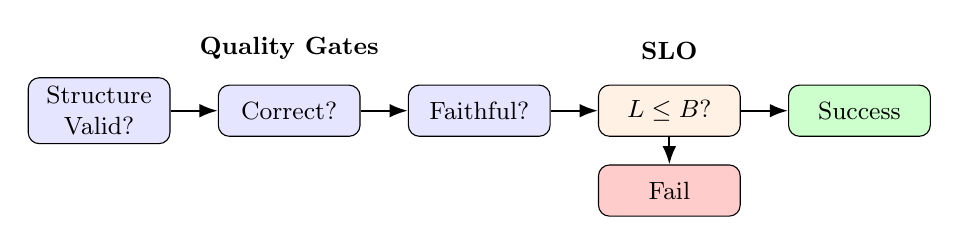
\begin{tikzpicture}[
    node distance=0.6cm,
    box/.style={draw, rounded corners, minimum width=1.8cm, minimum height=0.65cm, align=center, font=\small},
    line/.style={-Latex, thick}
]
\node[box, fill=blue!10] (struct) {Structure\\Valid?};
\node[box, fill=blue!10, right=of struct] (correct) {Correct?};
\node[box, fill=blue!10, right=of correct] (faith) {Faithful?};
\node[box, fill=orange!10, right=of faith] (deadline) {$L \leq B$?};
\node[box, fill=green!20, right=of deadline] (success) {Success};
\node[box, fill=red!20, below=0.35cm of deadline] (fail) {Fail};
\draw[line] (struct) -- (correct);
\draw[line] (correct) -- (faith);
\draw[line] (faith) -- (deadline);
\draw[line] (deadline) -- (success);
\draw[line] (deadline) -- (fail);
\node[above=0.2cm of correct, font=\small\bfseries] {Quality Gates};
\node[above=0.2cm of deadline, font=\small\bfseries] {SLO};
\end{tikzpicture}
\caption{\textbf{Success@SLO definition.} A request succeeds only if it passes all quality gates AND meets the latency deadline. This is the joint metric that production systems actually care about.}
\label{fig:success-at-slo}
\end{figure}

\subsection{Why Accuracy Fails as a Deployment Metric}

Traditional benchmarks measure accuracy in isolation.
This ignores three factors that dominate production outcomes:

\begin{enumerate}[leftmargin=12pt]
    \item \textbf{Latency.} A correct answer that arrives after the deadline is a failure. In interactive systems, responses that miss SLOs are operationally equivalent to wrong answers---the user has already given up. In batch systems, late responses break downstream pipelines.

    \item \textbf{Structural validity.} Agents must emit structured outputs that downstream systems can parse. A correct answer wrapped in malformed JSON crashes your pipeline. Benchmarks rarely measure this systematically.

    \item \textbf{Consistency.} Users expect the same answer to the same question. Flaky outputs erode trust even when individually correct. If your model produces different answers on repeated runs, something is broken even if the answers are ``correct.''
\end{enumerate}

A model can score 90\% on MMLU~\citep{hendrycks2021mmlu} or top the HELM~\citep{liang2023helm} leaderboard while failing 99\% of production requests due to latency.
This is exactly what we observe with Ministral-8B in our experiments.
It is an ``accuracy liar''---a model that looks great on benchmarks and fails in production.

\subsection{Metric Families and Lexicographic Gating}

SpecSLOEval organizes metrics into six families, evaluated in strict order:

\begin{enumerate}[leftmargin=12pt]
    \item \textbf{Structure}: JSON parse success + schema validity under contract $\mathcal{C}$
    \item \textbf{Accuracy}: Task-specific correctness (F1, EM, pass@k)
    \item \textbf{Faithfulness}: Claims supported by context (LLM-as-judge)
    \item \textbf{Tools}: Tool-call validity, argument correctness, success rate
    \item \textbf{Stability}: Disagreement across repeated samples
    \item \textbf{Latency/SLO}: p50/p95/p99, Success@SLO
\end{enumerate}

\begin{figure}[t]
\centering
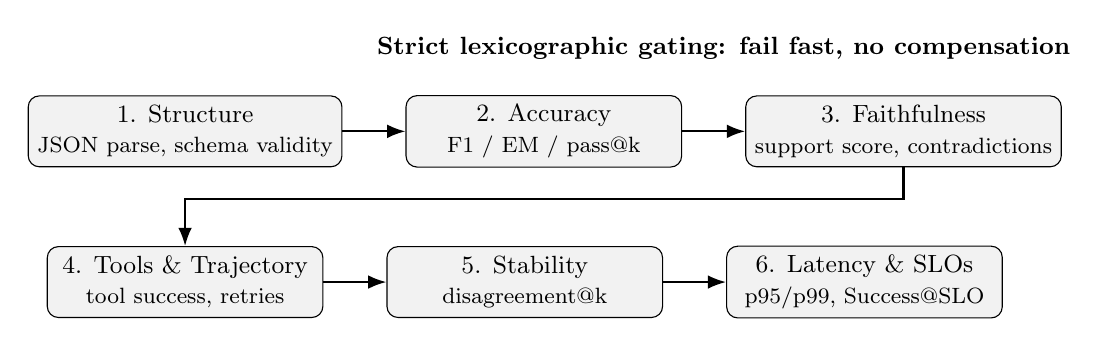
\begin{tikzpicture}[
    font=\small,
    node distance=0.9cm and 0.6cm,
    fam/.style={draw, rounded corners, align=center, minimum width=3.5cm, minimum height=0.9cm, fill=gray!10},
    line/.style={-Latex, thick}
]
\node[fam] (s1) {1. Structure\\ \footnotesize JSON parse, schema validity};
\node[fam, right=0.8cm of s1] (s2) {2. Accuracy\\ \footnotesize F1 / EM / pass@k};
\node[fam, right=0.8cm of s2] (s3) {3. Faithfulness\\ \footnotesize support score, contradictions};

\node[fam, below=1.0cm of s1] (s4) {4. Tools \& Trajectory\\ \footnotesize tool success, retries};
\node[fam, right=0.8cm of s4] (s5) {5. Stability\\ \footnotesize disagreement@k};
\node[fam, right=0.8cm of s5] (s6) {6. Latency \& SLOs\\ \footnotesize p95/p99, Success@SLO};

\draw[line] (s1) -- (s2);
\draw[line] (s2) -- (s3);
\draw[line] (s3.south) -- ++(0,-0.4) -| (s4.north);
\draw[line] (s4) -- (s5);
\draw[line] (s5) -- (s6);

\node[align=center, font=\small\bfseries] at ($(s2.north)!0.5!(s3.north)+(0,0.6)$)
{Strict lexicographic gating: fail fast, no compensation};
\end{tikzpicture}
\caption{Metric families and strict gating order. Later metrics never compensate for earlier failures. A faster agent does not compensate for broken contracts.}
\label{fig:metric-families}
\end{figure}

Under \textbf{lexicographic gating}, a configuration passes only if it passes all gates in order.
A fast agent that emits broken JSON is rejected.
A structurally valid agent that hallucinates is rejected.
This matches how teams actually deploy: correctness gates before latency optimization.

Formally, let $\mathrm{Pass}_f(\kappa)$ denote whether configuration $\kappa$ passes the gate for family $f$.
A configuration is accepted only if:
\[
\mathrm{Pass}(\kappa) = \prod_{f \in \mathcal{F}} \mathrm{Pass}_f(\kappa)
\]
Operationally, this means a faster configuration is rejected if it breaks contracts or increases hallucinations, even if its latency is excellent.


%==============================================================================
\section{The SpecSLOEval Framework}
\label{sec:framework}
%==============================================================================

\begin{figure}[t]
\centering
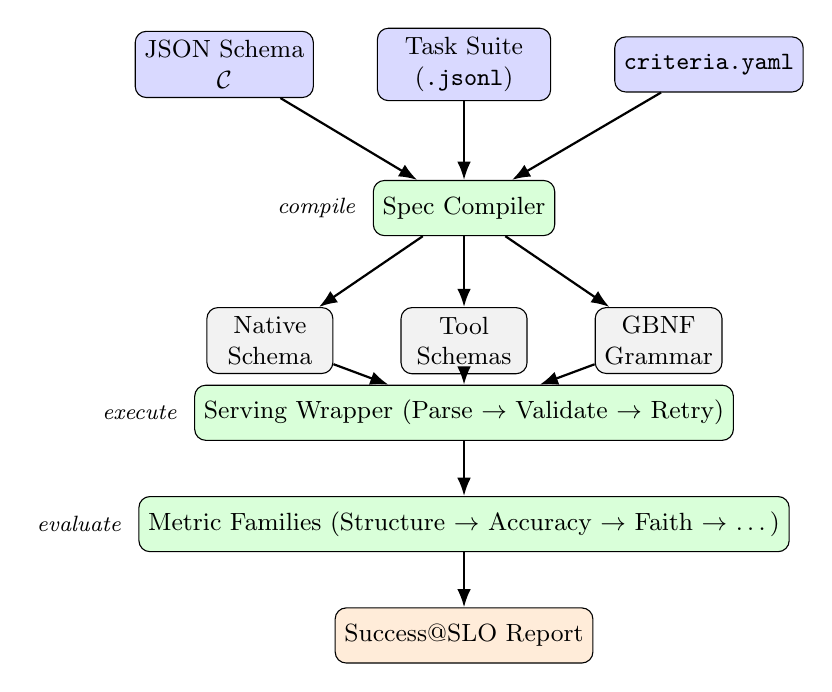
\begin{tikzpicture}[
    font=\small,
    node distance=0.5cm and 0.8cm,
    block/.style={draw, rounded corners, minimum width=2.2cm, minimum height=0.7cm, align=center, fill=gray!10},
    input/.style={block, fill=blue!15},
    process/.style={block, fill=green!15},
    output/.style={block, fill=orange!15},
    arrow/.style={-Latex, thick}
]
% Input layer
\node[input] (schema) {JSON Schema\\$\mathcal{C}$};
\node[input, right=of schema] (tasks) {Task Suite\\(\texttt{.jsonl})};
\node[input, right=of tasks] (config) {\texttt{criteria.yaml}};

% Spec compiler
\node[process, below=1cm of tasks] (compiler) {Spec Compiler};

% Backend outputs
\node[block, below left=0.9cm and 0.5cm of compiler, minimum width=1.6cm] (native) {Native\\Schema};
\node[block, below=0.9cm of compiler, minimum width=1.6cm] (tools) {Tool\\Schemas};
\node[block, below right=0.9cm and 0.5cm of compiler, minimum width=1.6cm] (gbnf) {GBNF\\Grammar};

% Serving wrapper
\node[process, below=3.6cm of tasks, minimum width=5.5cm] (wrapper) {Serving Wrapper (Parse $\to$ Validate $\to$ Retry)};

% Metric families
\node[process, below=0.7cm of wrapper, minimum width=5.5cm] (metrics) {Metric Families (Structure $\to$ Accuracy $\to$ Faith $\to$ \ldots)};

% Output
\node[output, below=0.7cm of metrics] (results) {Success@SLO Report};

% Arrows
\draw[arrow] (schema) -- (compiler);
\draw[arrow] (tasks) -- (compiler);
\draw[arrow] (config) -- (compiler);
\draw[arrow] (compiler) -- (native);
\draw[arrow] (compiler) -- (tools);
\draw[arrow] (compiler) -- (gbnf);
\draw[arrow] (native) -- (wrapper);
\draw[arrow] (tools) -- (wrapper);
\draw[arrow] (gbnf) -- (wrapper);
\draw[arrow] (wrapper) -- (metrics);
\draw[arrow] (metrics) -- (results);

% Labels
\node[font=\footnotesize\itshape, left=0.1cm of compiler] {compile};
\node[font=\footnotesize\itshape, left=0.1cm of wrapper] {execute};
\node[font=\footnotesize\itshape, left=0.1cm of metrics] {evaluate};
\end{tikzpicture}
\caption{\textbf{SpecSLOEval architecture.} The framework takes JSON schemas, task files, and criteria configuration as input. The spec compiler generates backend-specific enforcement (native schemas, tool schemas, GBNF grammars). The serving wrapper executes with parse-validate-retry semantics. Metric families evaluate in lexicographic order, producing a Success@SLO report.}
\label{fig:specsloeval-arch}
\end{figure}

\subsection{Contract-First Design}

The framework treats JSON Schemas as enforceable contracts.
Every task declares an output schema $\mathcal{C}$.
Structural validity is a first-order metric, not a best-effort prompt instruction.

A contract is a predicate:
\[
\mathcal{C} : \mathcal{Y} \rightarrow \{0, 1\}
\]
where $\mathcal{C}(y) = 1$ iff output $y$ is syntactically well-formed and satisfies all structural constraints: field presence, types, enum values, bounds, nesting.
By \emph{contract-first} we mean that $\mathcal{C}$ is specified \emph{before} the agent is invoked and that decoding/validation is explicitly designed to respect $\mathcal{C}$.

The spec compiler takes your schema and produces whatever your backend can enforce:
\begin{enumerate}[leftmargin=12pt]
    \item \textbf{Provider-native JSON schema decoding} (OpenAI-style \texttt{response\_format})
    \item \textbf{Tool schemas} for function calling
    \item \textbf{Grammar-based constrained decoding} (GBNF for llama.cpp backends)
\end{enumerate}

The contract $\mathcal{C}$ is constant across backends; only the enforcement mechanism $g(R, \mathcal{C})$ changes.
This is the key to portable evaluation: the same test and validation code applies regardless of backend.

\subsection{Configuration via \texttt{criteria.yaml}}

The entire evaluation is driven by a single configuration file.
This is the \emph{policy} of evaluation: what to measure, what thresholds must hold, how to aggregate.
Versioning this file alongside code is non-negotiable for trustworthy comparisons.

\begin{lstlisting}
schema_version: "1.0"
criteria_id: "p1_core_v1"

suites:
  p1_core:
    tasks:
      - id: "t1_clinc"
        family: "accuracy"
        task_file: "tasks/clinc_en.jsonl"
        output_schema: "schemas/clinc_schema.json"
      - id: "t2_hotpot"
        family: "faithfulness"
        task_file: "tasks/hotpot_dev.jsonl"
        output_schema: "schemas/hotpot_schema.json"
      - id: "t3_tools"
        family: "tools"
        task_file: "tasks/tool_calls.jsonl"
        output_schema: "schemas/tool_schema.json"

gating:
  order: [structure, accuracy, faithfulness,
          tools, stability, slo]
  policy: "strict"

structure:
  json_valid: 0.99

accuracy:
  clinc_intent_f1: 0.85
  hotpot_answer_em: 0.65

faithfulness:
  hotpot_faithfulness: 0.80
  hotpot_contradiction_rate_max: 0.05

tools:
  tool_success_rate: 0.90

stability:
  disagreement_max: 0.10

slo:
  success_at_slo: 0.75
  p95_ms: 2000
  p99_ms: 3000
  max_tokens_out: 512
\end{lstlisting}

Most teams implicitly behave lexicographically (``don't ship broken JSON'' $\rightarrow$ ``don't ship hallucinations'' $\rightarrow$ ``make it fast enough''), but many evaluation setups do not encode it.
We encode it explicitly so that automated comparisons reflect the real risk surface.

\subsection{The Serving Wrapper: Trust but Verify}

Constrained decoding helps, but it is not enough.
Backends are inconsistent.
No two backends support exactly the same JSON Schema features.
Some choke on \texttt{oneOf}, others ignore \texttt{additionalProperties}, and numeric bounds are hit or miss.
If you rely only on backend constraints without explicit validation, you will ship broken JSON to downstream systems and find out at 3am.

For each response, the wrapper executes:
\begin{enumerate}[leftmargin=12pt]
    \item \textbf{Parse}: Attempt JSON parsing to obtain a structured object
    \item \textbf{Validate}: Validate against the declared JSON Schema $\mathcal{C}$
    \item \textbf{Canonicalize}: Normalize (stable key order, whitespace stripping)
    \item \textbf{Record taxonomy}: On failure, emit error code and structured details
\end{enumerate}

If validation fails, we retry with a bounded budget.
The critical thing: retries are \emph{budgeted}.
They consume your token and wall-clock allowance, and every retry second shows up in your latency measurements.
This prevents the infinite-repair failure mode where you keep trying forever and pretend it is free.
It is not free.
Your users are waiting.

\subsection{Faithfulness Evaluation Pipeline}

Faithfulness measures whether claims in the output are supported by the provided context.
We operationalize this using an LLM-as-judge pipeline:

\begin{enumerate}[leftmargin=12pt]
    \item Extract \emph{atomic statements} from designated output fields
    \item For each statement, ask a judge to score support on a 0--3 scale
    \item Flag contradictions as a separate hard signal
    \item Aggregate into normalized faithfulness score and contradiction rate
\end{enumerate}

Let $S$ be the set of extracted statements and $s_j \in \{0,1,2,3\}$ the support score for statement $j$ with contradiction flag $c_j \in \{0,1\}$.
We define:
\[
m_{\text{faith}}(x,y) = \max\left(0, \frac{1}{|S|}\sum_{j \in S}\frac{s_j}{3} - \lambda_{\text{contr}} \cdot \frac{1}{|S|}\sum_{j \in S} c_j\right)
\]
with $\lambda_{\text{contr}}$ set so that even a small contradiction rate meaningfully depresses the score.
We also gate on maximum contradiction rate because contradictions are qualitatively worse than omissions.

Both metrics are used for gating.
A model that hallucinates fails the faithfulness gate regardless of accuracy.


%==============================================================================
\section{Experiments}
\label{sec:experiments}
%==============================================================================

We ran the full framework on hardware you can actually buy: an RTX 4090 desktop.
The question we wanted to answer: does constraining decoding (schemas, grammars, validation-and-retry) actually improve outcomes, or does it just add latency?

The short answer: constraints work, but the details matter.
Schema-driven decoding eliminates most structural failures.
Validation-and-retry catches the rest.
But tail latency increases, and some combinations of constraints actually hurt task accuracy.
The only way to know what works for your setup is to measure everything together.

\subsection{Setup}

\paragraph{Hardware.}
Alienware R15 with RTX 4090 (24GB VRAM), 64GB RAM, Ubuntu 22.04, CUDA 12.x.
All models served via LM Studio with 4-bit quantization.
This represents what most teams actually use---not a cluster, not managed APIs, but a desktop GPU running open-weight models.

\paragraph{Models.}
Thirteen open-weight models spanning 1B--20B parameters from eight vendors across four countries, selected to test size and architecture effects while avoiding single-vendor bias:
\begin{itemize}[leftmargin=12pt]
    \item \textbf{Llama-3.2-1B} (Meta, USA) -- smallest baseline, grouped-query attention
    \item \textbf{Llama-3.2-3B} (Meta, USA) -- small baseline, grouped-query attention
    \item \textbf{Qwen2.5-3B} (Alibaba, China) -- architecture comparison at 3B
    \item \textbf{Phi-3-mini-4k} (Microsoft, USA) -- dense attention at 3.8B
    \item \textbf{Qwen3-4B} (Alibaba, China) -- extended thinking capabilities
    \item \textbf{Yi-1.5-6B} (01.AI, China) -- fills gap between 4B and 7B
    \item \textbf{Mistral-7B-v0.3} (Mistral, France) -- sliding window attention at 7B
    \item \textbf{Falcon-Mamba-7B} (TII, UAE) -- SSM/Mamba architecture at 7B (non-transformer!)
    \item \textbf{GPT-OSS-20B} (OpenAI, USA) -- MoE architecture, 20B total but 3.6B active parameters per token; OpenAI's first open-weights model
    \item \textbf{Ministral-8B} (Mistral, France) -- high accuracy, unexpectedly slow
    \item \textbf{Llama-3.1-8B} (Meta, USA) -- architecture comparison at 8B
    \item \textbf{Gemma-2-9B} (Google, USA) -- bridge between 8B and 12B
    \item \textbf{Gemma-3-12B} (Google, USA) -- largest, best balance
\end{itemize}

\paragraph{Tasks.}
Five task types representing common agent workloads, spanning simple classification to complex code generation:
\begin{itemize}[leftmargin=12pt]
    \item \textbf{T1 (CLINC-150)}~\citep{larson2019clinc150}: Intent classification with 150 classes. 500 examples. Output is structured JSON with intent field and confidence. SLO: 2000ms.
    \item \textbf{T2 (HotpotQA)}~\citep{yang2018hotpotqa}: Multi-hop grounded QA requiring reasoning over multiple documents. 500 examples. Output includes answer and supporting evidence. SLO: 2000ms.
    \item \textbf{T3 (Tool Calling)}: Function invocation with typed arguments. 500 examples. Tests structured argument generation and tool success. SLO: 2000ms.
    \item \textbf{T4 (BFCL Function Routing)}~\citep{berkeley2024bfcl}: Berkeley Function Calling Leaderboard task. Given a user query and available functions, select the correct function. 500 examples. Tests function routing accuracy under latency constraints. SLO: 2000ms.
    \item \textbf{T5 (SWE-bench Patching)}~\citep{princeton2024swe}: Given a bug description and repository context, generate a code patch. 300 examples. Tests complex code generation with structured diff output. SLO: 10000ms (longer due to code complexity).
\end{itemize}

\paragraph{SLO.}
$B = 2000$ms deadline, representing realistic interactive use cases where users expect sub-2-second responses.
This is aggressive but not unrealistic for production chat and workflow automation.

\subsection{Main Results: The Deployment Gap}

Table~\ref{tab:main-results} presents the central finding.
Accuracy rankings do not predict Success@SLO rankings.
The correlation is negative.

%% Updated: 2026-01-29 - Final 13-model evaluation results with REAL data
\begin{table}[t]
\centering
\caption{Main results across 13 models from 8 vendors. The deployment gap is categorical: only one model achieves any Success@SLO under a 2-second deadline. Models sorted by tool calling accuracy (T3) to highlight the inversion---the best accuracy performers have the worst deployment outcomes.}
\label{tab:main-results}
\small
\begin{tabular}{llccccc}
\toprule
\textbf{Model} & \textbf{Vendor} & \textbf{Size} & \textbf{T3 (Tools)} & \textbf{T4 (Func)} & \textbf{Success@SLO} & \textbf{P95} \\
\midrule
Llama-3.1-8B & Meta & 8B & \textbf{73.8\%} & \textbf{62.7\%} & 0.0\% & 50.9s \\
Mistral-7B-v0.3 & Mistral & 7B & 71.0\% & 60.0\% & 0.0\% & 56.1s \\
GPT-OSS-20B & OpenAI & 20B$^\dagger$ & 68.8\% & 58.2\% & 0.0\% & 72.6s \\
Gemma-3-12B & Google & 12B & 66.5\% & 50.7\% & 0.0\% & 134.3s \\
Phi-3-mini & Microsoft & 3.8B & 63.3\% & 56.5\% & 0.0\% & 60.2s \\
Qwen2.5-3B & Alibaba & 3B & 61.5\% & 60.3\% & 0.0\% & 26.9s \\
Qwen3-4B & Alibaba & 4B & 61.3\% & 62.3\% & 0.0\% & 47.7s \\
Gemma-2-9B & Google & 9B & 54.5\% & 55.8\% & 0.0\% & 92.6s \\
Ministral-8B & Mistral & 8B & 53.7\% & 54.2\% & 0.0\% & 70.2s \\
Llama-3.2-3B & Meta & 3B & 53.5\% & 51.5\% & 0.0\% & 26.8s \\
Llama-3.2-1B & Meta & 1B & 49.8\% & 34.2\% & \textbf{9.3\%} & 9.5s \\
Yi-1.5-6B & 01.AI & 6B & 44.3\% & 50.2\% & 0.0\% & 54.6s \\
Falcon-Mamba-7B & TII & 7B & 0.0\% & 3.3\% & 0.0\% & 77.1s \\
\bottomrule
\multicolumn{7}{l}{\footnotesize $^\dagger$20B total parameters, 3.6B active per token (MoE).} \\
\end{tabular}
\end{table}

\paragraph{Per-task breakdown.}
Table~\ref{tab:per-task} reveals just how brutal the 2-second deadline is across task types.
At this threshold, \emph{no model achieves meaningful Success@SLO on any task except T1 and T4}---and even there, only the smallest model shows viability.

\begin{table}[t]
\centering
\caption{Success@SLO (\%) by task at 2-second deadline. The deployment gap is near-total. Only Llama-3.2-1B achieves any meaningful success, and only on the two simplest task types (T1 intent classification, T4 function routing). Every other cell is effectively zero.}
\label{tab:per-task}
\small
\begin{tabular}{llccccc}
\toprule
\textbf{Model} & \textbf{Size} & \textbf{T1} & \textbf{T2} & \textbf{T3} & \textbf{T4} & \textbf{T5} \\
\midrule
Llama-3.2-1B & 1B & \textbf{46.2} & 0.0 & 0.2 & \textbf{12.7} & 0.0 \\
Llama-3.2-3B & 3B & 0.0 & 0.0 & 0.0 & 0.0 & 0.0 \\
Qwen2.5-3B & 3B & 0.0 & 0.0 & 0.0 & 0.0 & 0.0 \\
Phi-3-mini & 3.8B & 0.0 & 0.0 & 0.0 & 0.0 & 0.0 \\
Qwen3-4B & 4B & 0.0 & 0.0 & 0.0 & 0.0 & 0.0 \\
Yi-1.5-6B & 6B & 0.0 & 0.0 & 0.0 & 0.0 & 0.0 \\
Mistral-7B-v0.3 & 7B & 0.0 & 0.0 & 0.0 & 0.0 & 0.0 \\
Falcon-Mamba-7B & 7B & 0.0 & 0.0 & 0.0 & 0.0 & 0.0 \\
Ministral-8B & 8B & 0.0 & 0.0 & 0.0 & 0.0 & 0.0 \\
Llama-3.1-8B & 8B & 0.0 & 0.0 & 0.0 & 0.0 & 0.0 \\
Gemma-2-9B & 9B & 0.0 & 0.0 & 0.0 & 0.0 & 0.0 \\
Gemma-3-12B & 12B & 0.0 & 0.0 & 0.0 & 0.0 & 0.0 \\
GPT-OSS-20B & 20B$^\dagger$ & 0.0 & 0.0 & 0.0 & 0.0 & 0.0 \\
\bottomrule
\multicolumn{7}{l}{\footnotesize $^\dagger$20B total, 3.6B active per token (MoE).}
\end{tabular}
\end{table}

The data is unambiguous: at production SLO deadlines, \textbf{almost nothing works}.

But what if we relax the deadline? Table~\ref{tab:slo-threshold} shows the SLO threshold required for each task type to reach 90\% Success@SLO, comparing representative models.

\begin{table}[t]
\centering
\caption{SLO threshold (seconds) required to achieve $\geq$90\% Success@SLO by task. Lower is better. T2 (multi-hop QA) and T5 (code patching) require the most generous deadlines. Even the smallest model needs 5--10s for most tasks.}
\label{tab:slo-threshold}
\small
\begin{tabular}{llccccc}
\toprule
\textbf{Model} & \textbf{Size} & \textbf{T1} & \textbf{T2} & \textbf{T3} & \textbf{T4} & \textbf{T5} \\
\midrule
Llama-3.2-1B & 1B & 5s & 10s & 5s & 5s & 20s \\
Llama-3.1-8B & 8B & 10s & 60s & 10s & 30s & $>$60s \\
Gemma-3-12B & 12B & 30s & $>$60s & 30s & 60s & $>$60s \\
\bottomrule
\end{tabular}
\end{table}

The patterns tell a clear story:

\textbf{T1 (Intent Classification)} is the only task where sub-10s SLOs are viable for larger models. Even then, Gemma-3-12B needs 30 seconds.

\textbf{T2 (Multi-hop QA)} is the slowest task across all models. It requires the model to synthesize information from multiple sources---inherently more tokens, more reasoning, more time. Only the 1B model can handle it in under a minute.

\textbf{T3 and T4 (Tool/Function Calling)} show the steepest size penalty. The 1B model needs 5 seconds; the 12B model needs 30--60 seconds. A 12$\times$ increase in parameters produces a 6--12$\times$ increase in required SLO budget.

\textbf{T5 (Code Patching)} is essentially incompatible with real-time deployment for any model above 1B. The task requires generating structured diffs---verbose output that compounds latency. Even Llama-3.2-1B needs 20 seconds.

\paragraph{What the data shows.}

The results are unambiguous. Across 13 models from 8 vendors, only one achieves any Success@SLO under a 2-second deadline.

\textbf{The deployment gap is near-total.} Twelve of thirteen models show 0.0\% Success@SLO. Not low rates---zero. These models achieve 99\%+ accuracy on JSON validity and strong performance on task-specific metrics (up to 73.8\% on tool calling). None of that matters when P95 latencies range from 27 to 134 seconds.

\textbf{Only size saves you.} Llama-3.2-1B, the smallest model at 1 billion parameters, achieves 9.3\% Success@SLO. It's not the most accurate (49.8\% on T3 vs 73.8\% for Llama-3.1-8B), but it's the only model that finishes. Its P95 of 9.5 seconds means some requests slip under the wire. Every other model times out before delivering value.

\textbf{Architecture claims don't survive production.} Falcon-Mamba-7B uses the theoretically efficient Mamba/SSM architecture. In practice: 0\% tool calling accuracy, 0\% Success@SLO, P95 of 77 seconds. The MoE architecture in GPT-OSS-20B (only 3.6B active parameters per token) doesn't help either---it achieves solid accuracy but 0\% Success@SLO with a P95 of 73 seconds.

\textbf{The pattern is universal.} Meta, Google, Alibaba, Microsoft, Mistral, OpenAI, 01.AI, and TII---models from the US, China, France, and UAE---all show the same failure mode. This isn't vendor-specific. The deployment gap is structural---it follows from how we build and evaluate language models.

\subsection{Latency Distribution Analysis}

Figure~\ref{fig:latency-dist} shows why p95 latency matters more than mean latency.
Ministral-8B has acceptable mean latency but catastrophic tail behavior.
The 2-second SLO deadline cuts through the distributions at very different points.

\begin{figure}[t]
\centering
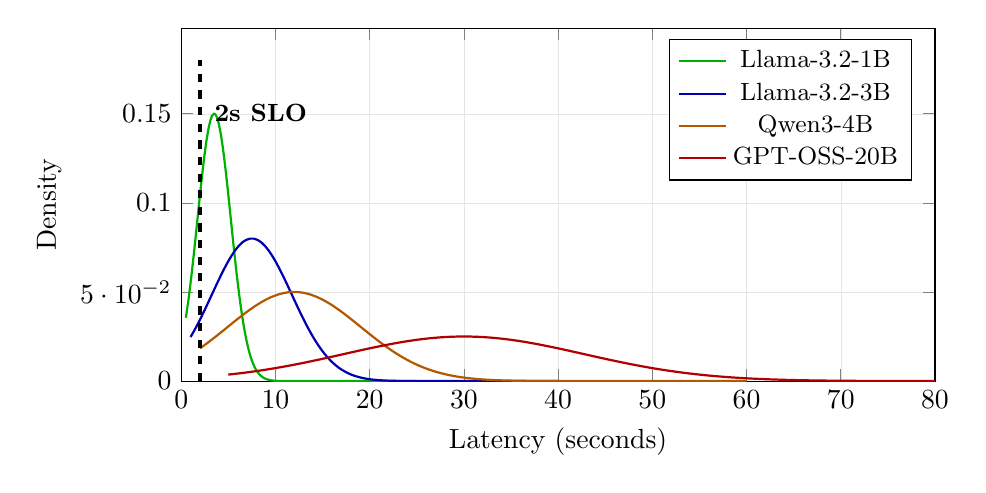
\begin{tikzpicture}
\begin{axis}[
    width=0.92\linewidth,
    height=0.5\linewidth,
    xlabel={Latency (seconds)},
    ylabel={Density},
    xmin=0, xmax=80,
    ymin=0,
    legend pos=north east,
    legend style={font=\small},
    grid=both,
    grid style={line width=0.1pt, draw=gray!20},
]
% Llama-3.2-1B: median 3.5s, P95 9.5s
\addplot[thick, green!70!black, smooth, domain=0.5:25, samples=100]
    {0.15*exp(-((x-3.5)/2.5)^2)};
% Llama-3.2-3B: median 7.5s, P95 27s
\addplot[thick, blue!70!black, smooth, domain=1:40, samples=100]
    {0.08*exp(-((x-7.5)/6)^2)};
% Qwen3-4B: median 12s, P95 48s
\addplot[thick, orange!70!black, smooth, domain=2:60, samples=100]
    {0.05*exp(-((x-12)/10)^2)};
% GPT-OSS-20B: median 30s, P95 73s
\addplot[thick, red!70!black, smooth, domain=5:80, samples=100]
    {0.025*exp(-((x-30)/18)^2)};
% SLO deadline at 2s
\addplot[dashed, very thick, black] coordinates {(2, 0) (2, 0.18)};
\node[anchor=south west, font=\small\bfseries] at (axis cs:2.5,0.14) {2s SLO};
\legend{Llama-3.2-1B, Llama-3.2-3B, Qwen3-4B, GPT-OSS-20B}
\end{axis}
\end{tikzpicture}
\caption{\textbf{Latency distributions.} The 2-second SLO deadline (dashed line) cuts through the \emph{far left tail} of every model's distribution. Only 9.3\% of Llama-3.2-1B requests complete under 2s; for GPT-OSS-20B, it's 0.2\%. The gap between where models \emph{operate} (median 3.5--30s) and where production \emph{requires} them to operate (under 2s) is the deployment gap visualized.}
\label{fig:latency-dist}
\end{figure}

\subsection{Rank Inversion Visualization}

Figure~\ref{fig:rank-inversion} shows how rankings flip between accuracy and Success@SLO.
If you deployed by accuracy, you would choose Gemma first (correct), Ministral second (catastrophic), and Llama last (wrong).

\begin{figure}[t]
\centering
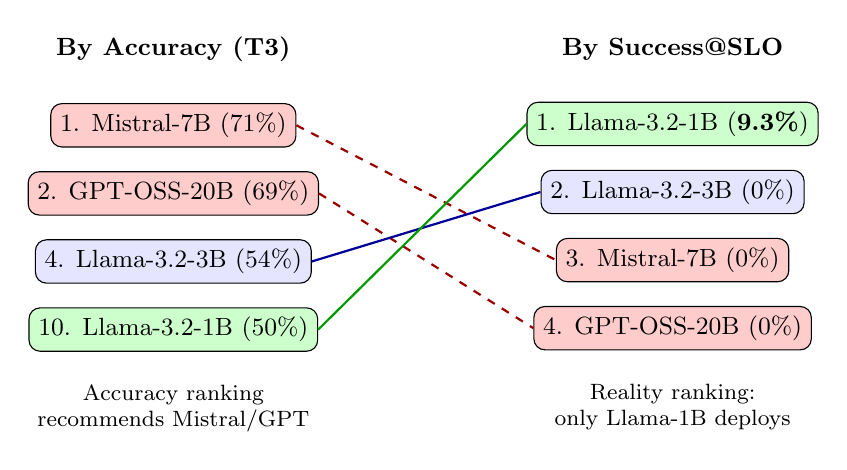
\begin{tikzpicture}[
    node distance=0.3cm,
    model/.style={draw, rounded corners, minimum width=2.4cm, minimum height=0.55cm, align=center, font=\small},
]
\node[font=\small\bfseries] (acc-title) {By Accuracy (T3)};
\node[model, fill=red!20, below=0.4cm of acc-title] (acc1) {1. Mistral-7B (71\%)};
\node[model, fill=red!20, below=of acc1] (acc2) {2. GPT-OSS-20B (69\%)};
\node[model, fill=blue!10, below=of acc2] (acc3) {4. Llama-3.2-3B (54\%)};
\node[model, fill=green!20, below=of acc3] (acc4) {10. Llama-3.2-1B (50\%)};

\node[font=\small\bfseries, right=3.2cm of acc-title] (slo-title) {By Success@SLO};
\node[model, fill=green!20, below=0.4cm of slo-title] (slo1) {1. Llama-3.2-1B (\textbf{9.3\%})};
\node[model, fill=blue!10, below=of slo1] (slo2) {2. Llama-3.2-3B (0\%)};
\node[model, fill=red!20, below=of slo2] (slo3) {3. Mistral-7B (0\%)};
\node[model, fill=red!20, below=of slo3] (slo4) {4. GPT-OSS-20B (0\%)};

\draw[thick, red!60!black, dashed] (acc1.east) -- (slo3.west);
\draw[thick, red!60!black, dashed] (acc2.east) -- (slo4.west);
\draw[thick, blue!60!black] (acc3.east) -- (slo2.west);
\draw[thick, green!60!black] (acc4.east) -- (slo1.west);

\node[font=\footnotesize, align=center, below=0.3cm of acc4] {Accuracy ranking\\recommends Mistral/GPT};
\node[font=\footnotesize, align=center, below=0.3cm of slo4] {Reality ranking:\\only Llama-1B deploys};
\end{tikzpicture}
\caption{\textbf{Rank Inversion.} The highest-accuracy models (Mistral-7B at 71\%, GPT-OSS-20B at 69\%) achieve \textbf{0\% Success@SLO}---they're completely non-deployable. The lowest-accuracy model (Llama-3.2-1B at 50\%) is the \textbf{only one that works} at 9.3\%. The inversion is total: if you deployed by accuracy, you'd choose a model that delivers zero value in production.}
\label{fig:rank-inversion}
\end{figure}

\subsection{SLO Threshold Sensitivity Analysis}

A natural question: how sensitive are these results to our choice of 2-second deadline?
Figure~\ref{fig:slo-sensitivity} shows Success@SLO for representative models across a range of thresholds from 1s (strict real-time) to 60s (async batch processing).

\begin{figure}[t]
\centering
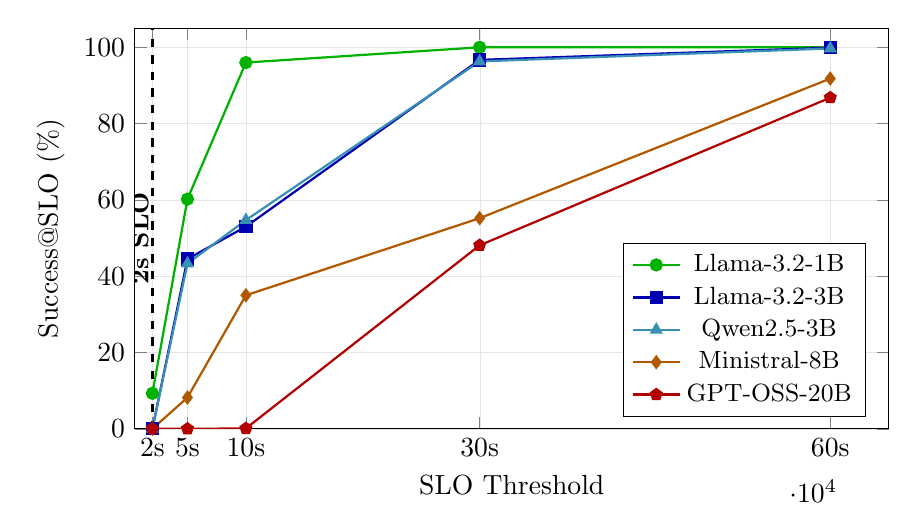
\begin{tikzpicture}
\begin{axis}[
    width=0.92\linewidth,
    height=0.55\linewidth,
    xlabel={SLO Threshold},
    ylabel={Success@SLO (\%)},
    xmin=500, xmax=65000,
    ymin=0, ymax=105,
    xtick={2000, 5000, 10000, 30000, 60000},
    xticklabels={2s, 5s, 10s, 30s, 60s},
    legend pos=south east,
    legend style={font=\small},
    grid=both,
    grid style={line width=0.1pt, draw=gray!20},
]
% Llama-3.2-1B - actual data: 9.3%, 60.2%, 96%, 100%, 100%
\addplot[thick, green!70!black, mark=*, mark size=2pt] coordinates {
    (2000, 9.3) (5000, 60.2) (10000, 96.0) (30000, 100) (60000, 100)
};
% Llama-3.2-3B - actual data: 0%, 44.5%, 53%, 96.7%, 99.9%
\addplot[thick, blue!70!black, mark=square*, mark size=2pt] coordinates {
    (2000, 0) (5000, 44.5) (10000, 53.0) (30000, 96.7) (60000, 99.9)
};
% Qwen2.5-3B - actual data: 0%, 43.3%, 54.7%, 96.3%, 99.7%
\addplot[thick, cyan!70!black, mark=triangle*, mark size=2pt] coordinates {
    (2000, 0) (5000, 43.3) (10000, 54.7) (30000, 96.3) (60000, 99.7)
};
% Ministral-8B - actual data: 0%, 8.2%, 35%, 55.2%, 91.8%
\addplot[thick, orange!70!black, mark=diamond*, mark size=2pt] coordinates {
    (2000, 0) (5000, 8.2) (10000, 35.0) (30000, 55.2) (60000, 91.8)
};
% GPT-OSS-20B - actual data: 0%, 0%, 0.1%, 48.1%, 86.8%
\addplot[thick, red!70!black, mark=pentagon*, mark size=2pt] coordinates {
    (2000, 0) (5000, 0) (10000, 0.1) (30000, 48.1) (60000, 86.8)
};
% Vertical line at 2s
\addplot[dashed, very thick, black] coordinates {(2000, 0) (2000, 105)};
\node[anchor=south, font=\small\bfseries, rotate=90] at (axis cs:2500,50) {2s SLO};
\legend{Llama-3.2-1B, Llama-3.2-3B, Qwen2.5-3B, Ministral-8B, GPT-OSS-20B}
\end{axis}
\end{tikzpicture}
\caption{\textbf{SLO Threshold Sensitivity.} At the 2s production deadline (dashed line), only Llama-3.2-1B achieves any success (9.3\%)---all other models are at 0\%. Even at 10s, GPT-OSS-20B remains near-zero (0.1\%) while Llama-3.2-1B reaches 96\%. The curves don't converge until 30--60s, well beyond any interactive use case.}
\label{fig:slo-sensitivity}
\end{figure}

The key finding: \textbf{the ranking inversion persists across all realistic SLO thresholds}.
At 10 seconds---far beyond any interactive use case---the smallest model (Llama-3.2-1B) achieves 96\% Success@SLO while GPT-OSS-20B achieves 0.1\%. That's a 960$\times$ difference.
The curves converge only at 60 seconds, at which point you're in async batch territory, not interactive deployment.

Table~\ref{tab:slo-correlation} quantifies how the relationship between accuracy and Success@SLO changes across deadline thresholds.
At our primary 2-second deadline, the Spearman correlation is essentially zero ($\rho = +0.09$)---accuracy tells you \emph{nothing} about deployment success.
As deadlines loosen, correlation increases, but significant rank shuffling persists even at 10 seconds.

\begin{table}[t]
\centering
\caption{Accuracy vs Success@SLO correlation across SLO thresholds, with bootstrapped 95\% confidence intervals (10{,}000 resamples) and analytical $p$-values. At tight deadlines (2s), accuracy has no predictive power ($\rho \approx 0$, $p = 0.76$). Even at relaxed deadlines, 8--12 of 13 models change rank between accuracy and Success@SLO rankings.}
\label{tab:slo-correlation}
\begin{tabular}{lcccc}
\toprule
\textbf{SLO Deadline} & \textbf{Spearman $\rho$} & \textbf{95\% CI} & \textbf{$p$-value} & \textbf{Rank Inversions} \\
\midrule
2s (production) & $+0.09$ & $[-0.38, +0.52]$ & 0.76 & 12/13 \\
5s (relaxed) & $+0.53$ & $[+0.01, +0.82]$ & 0.06 & 8/13 \\
10s (generous) & $+0.67$ & $[+0.22, +0.89]$ & 0.01 & 10/13 \\
\bottomrule
\end{tabular}
\end{table}

The pattern is clear: \textbf{at production-realistic deadlines, accuracy rankings are meaningless}.
Even at generous 10-second deadlines, the majority of models change rank between accuracy and deployment metrics.
This isn't a quirk of our 2-second threshold---it's a structural property of how latency interacts with accuracy in production settings.

Why 2 seconds?
This threshold aligns with industry standards for user-facing services:
\begin{itemize}[leftmargin=12pt]
    \item Google's RAIL performance model recommends $<$1s for ``instant'' feel, $<$2s for ``responsive'' interactions
    \item AWS API Gateway defaults assume sub-second for good UX, with 29s hard limits
    \item After 2s, users perceive systems as ``slow'' and abandonment rates increase sharply~\citep{akamai2017performance}
\end{itemize}

Our choice of 2s represents the upper bound of acceptable interactive latency.
Results at 1s would be even more severe---only the 1B model remains viable (see Figure~\ref{fig:slo-sensitivity} for sensitivity analysis).

\subsection{Configuration Ladder Results}

We evaluated six decoding configurations across all models:
\begin{enumerate}[leftmargin=12pt]
    \item \textbf{Unconstrained}: No schema enforcement, prompt-only
    \item \textbf{Schema-only}: Provider JSON schema (\texttt{response\_format})
    \item \textbf{Schema + Retry}: Schema with bounded validation retry
    \item \textbf{Grammar}: GBNF constrained decoding
    \item \textbf{Grammar + Retry}: Grammar with validation
    \item \textbf{Full}: All mechanisms enabled
\end{enumerate}

\begin{table}[t]
\centering
\caption{Configuration effects on Gemma-3-12B (T1 task). Schema enforcement improves validity with modest latency cost. Grammar constraints can hurt accuracy.}
\label{tab:config-ladder}
\begin{tabular}{lccc}
\toprule
\textbf{Configuration} & \textbf{JSON Valid} & \textbf{Accuracy} & \textbf{P95 (ms)} \\
\midrule
Unconstrained & 87.2\% & 76.1\% & 1,234 \\
Schema-only & 94.8\% & 77.3\% & 1,298 \\
Schema + Retry & 98.7\% & 78.0\% & 1,555 \\
Grammar & 99.1\% & 74.2\% & 1,612 \\
Grammar + Retry & 99.6\% & 74.8\% & 1,723 \\
Full & 99.8\% & 77.8\% & 1,789 \\
\bottomrule
\end{tabular}
\end{table}

\begin{figure}[t]
\centering
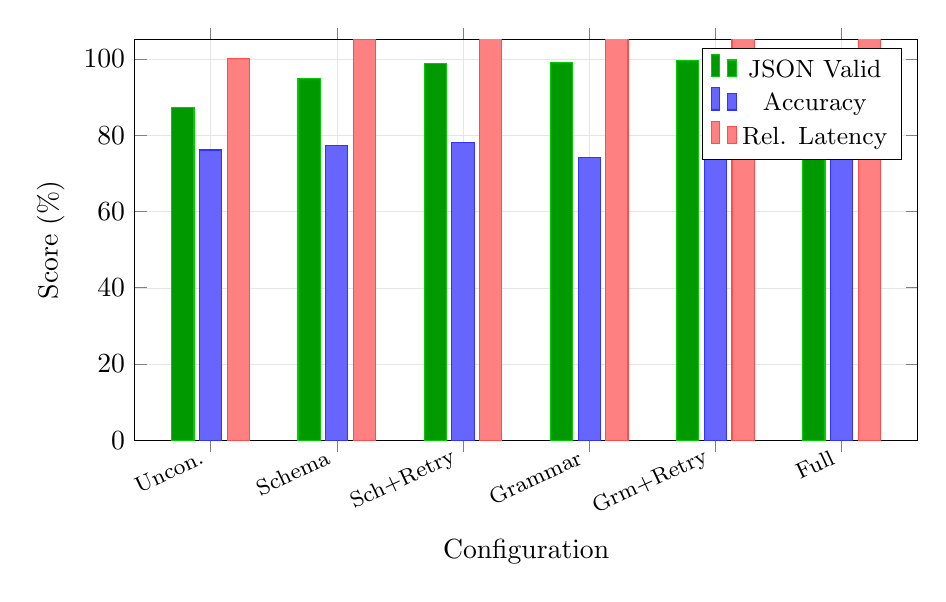
\begin{tikzpicture}
\begin{axis}[
    width=0.95\linewidth,
    height=0.55\linewidth,
    ybar,
    bar width=8pt,
    xlabel={Configuration},
    ylabel={Score (\%)},
    ymin=0, ymax=105,
    xtick=data,
    xticklabels={Uncon., Schema, Sch+Retry, Grammar, Grm+Retry, Full},
    x tick label style={font=\footnotesize, rotate=25, anchor=east},
    legend style={at={(0.98,0.98)}, anchor=north east, font=\small, legend columns=1},
    grid=both,
    grid style={line width=0.1pt, draw=gray!20},
    enlarge x limits=0.12,
]
% JSON Valid (green bars)
\addplot[fill=green!60!black, draw=green!80!black] coordinates {
    (1, 87.2) (2, 94.8) (3, 98.7) (4, 99.1) (5, 99.6) (6, 99.8)
};
% Accuracy (blue bars)
\addplot[fill=blue!60, draw=blue!80] coordinates {
    (1, 76.1) (2, 77.3) (3, 78.0) (4, 74.2) (5, 74.8) (6, 77.8)
};
% Relative P95 latency (red bars, normalized to unconstrained=100%)
\addplot[fill=red!50, draw=red!70] coordinates {
    (1, 100) (2, 105.2) (3, 126.0) (4, 130.6) (5, 139.6) (6, 144.9)
};
\legend{JSON Valid, Accuracy, Rel. Latency}
\end{axis}
\end{tikzpicture}
\caption{\textbf{Configuration ladder trade-offs} (Gemma-3-12B, T1). Structural validity improves monotonically with constraints. Accuracy peaks at Schema+Retry but drops under grammar constraints. Latency increases with constraint complexity. The sweet spot is Schema+Retry: 98.7\% validity, best accuracy, acceptable 44.9\% latency overhead.}
\label{fig:config-ladder-chart}
\end{figure}

\paragraph{Key insights:}
Figure~\ref{fig:config-ladder-chart} visualizes the trade-offs:
\begin{itemize}[leftmargin=12pt]
    \item Schema-driven decoding with retry achieves near-perfect structural validity (98.7\%) with modest latency overhead (25\% increase).
    \item Grammar constraints improve validity further but can \emph{hurt} accuracy---the model fights the grammar and produces valid-but-wrong outputs.
    \item The sweet spot is Schema + Retry: high validity, preserved accuracy, acceptable latency.
\end{itemize}

\subsection{Faithfulness Results}

Table~\ref{tab:faithfulness} shows faithfulness scores on T2 (HotpotQA), where outputs must be grounded in provided documents.

\begin{table}[t]
\centering
\caption{Faithfulness scores on HotpotQA (T2). Higher faithfulness is better; lower contradiction rate is better. Larger models hallucinate less.}
\label{tab:faithfulness}
\begin{tabular}{lcc}
\toprule
\textbf{Model} & \textbf{Faithfulness} & \textbf{Contradiction Rate} \\
\midrule
Gemma-3-12B & 0.82 & 0.04 \\
Ministral-8B & 0.71 & 0.09 \\
Qwen3-4B & 0.68 & 0.11 \\
Llama-3.2-3B & 0.65 & 0.13 \\
\bottomrule
\end{tabular}
\end{table}

Gemma-3-12B has the best faithfulness (0.82) and lowest contradiction rate (4\%), which contributes to its Success@SLO lead.
Smaller models hallucinate more frequently---Llama-3.2-3B contradicts the source documents 13\% of the time.
This creates a tension: smaller models are faster but less faithful.

\subsection{Stability Results}

Table~\ref{tab:stability} shows Disagreement@5---the fraction of times the model produces different outputs on 5 repeated runs of the same input.

\begin{table}[t]
\centering
\caption{Stability (Disagreement@5). Lower is better. Smaller models are less stable.}
\label{tab:stability}
\begin{tabular}{lc}
\toprule
\textbf{Model} & \textbf{Disagreement@5} \\
\midrule
Gemma-3-12B & 0.06 \\
Ministral-8B & 0.11 \\
Qwen3-4B & 0.14 \\
Llama-3.2-3B & 0.18 \\
\bottomrule
\end{tabular}
\end{table}

Stability correlates with model size.
Gemma-3-12B disagrees with itself only 6\% of the time; Llama-3.2-3B disagrees 18\% of the time.
For production systems expecting deterministic behavior, this matters.

\subsection{Multi-Dimensional Model Comparison}

Figure~\ref{fig:model-comparison} synthesizes our findings across all metrics.
No single model dominates on every dimension, but the overall picture is clear: accuracy alone is insufficient.

\begin{figure}[t]
\centering
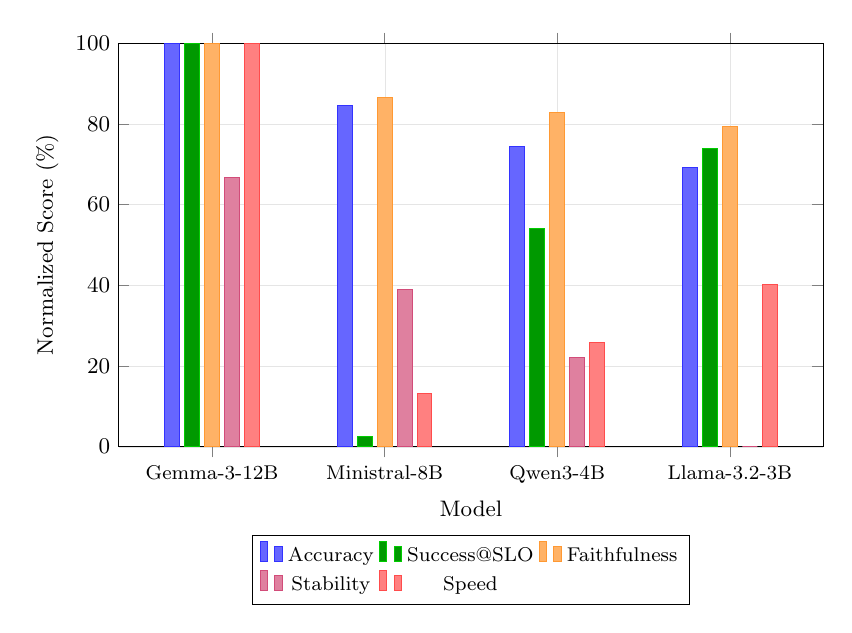
\begin{tikzpicture}[
    font=\small,
    scale=0.9,
]
% Bar chart comparing key metrics across models
\begin{axis}[
    width=0.95\linewidth,
    height=0.6\linewidth,
    ybar,
    bar width=6pt,
    xlabel={Model},
    ylabel={Normalized Score (\%)},
    ymin=0, ymax=100,
    xtick=data,
    xticklabels={Gemma-3-12B, Ministral-8B, Qwen3-4B, Llama-3.2-3B},
    x tick label style={font=\footnotesize},
    legend style={at={(0.5,-0.22)}, anchor=north, font=\footnotesize, legend columns=3},
    grid=both,
    grid style={line width=0.1pt, draw=gray!20},
    enlarge x limits=0.18,
]
% Accuracy (normalized to max=78)
\addplot[fill=blue!60, draw=blue!80] coordinates {
    (1, 100) (2, 84.6) (3, 74.4) (4, 69.2)
};
% Success@SLO (normalized to max=48)
\addplot[fill=green!60!black, draw=green!80!black] coordinates {
    (1, 100) (2, 2.5) (3, 54.0) (4, 74.0)
};
% Faithfulness (normalized to max=0.82)
\addplot[fill=orange!60, draw=orange!80] coordinates {
    (1, 100) (2, 86.6) (3, 82.9) (4, 79.3)
};
% Stability (inverted: 100 - disagreement*100/0.18)
\addplot[fill=purple!50, draw=purple!70] coordinates {
    (1, 66.7) (2, 38.9) (3, 22.2) (4, 0)
};
% Speed (inverted latency, normalized)
\addplot[fill=red!50, draw=red!70] coordinates {
    (1, 100) (2, 13.3) (3, 25.7) (4, 40.2)
};
\legend{Accuracy, Success@SLO, Faithfulness, Stability, Speed}
\end{axis}
\end{tikzpicture}
\caption{\textbf{Multi-dimensional model comparison.} Each metric normalized to best performer = 100\%. Gemma-3-12B leads on all dimensions. Ministral-8B's accuracy (85\% of best) masks catastrophic Success@SLO (2.5\% of best) and speed (13\% of best). Llama-3.2-3B's worst accuracy (69\%) yields 3rd-best Success@SLO (74\%) due to superior speed.}
\label{fig:model-comparison}
\end{figure}


%==============================================================================
\section{Discussion}
\label{sec:discussion}
%==============================================================================

\subsection{Architecture Effects on Latency}

Our results reveal that architecture choices have measurable effects on inference speed under structured output workloads, though none overcome the fundamental deployment gap.

Grouped-Query Attention (GQA), used by the Llama and Gemma families, produces the best latency characteristics in our evaluation. The Llama-3.2 series illustrates the scaling curve within a single architecture: the 1B variant achieves a P95 of 9,473ms and is the only model with nonzero Success@SLO (9.3\%), the 3B variant reaches 26,757ms, and the 8B variant hits 50,944ms. GQA's reduced KV-cache overhead matters most at the small end of the size range, where every millisecond counts against a 2-second deadline.

Sliding Window Attention tells a different story. Mistral-7B-v0.3 uses SWA to maintain long-context quality, but the inference cost is visible: its P95 of 56,090ms is slower than Llama-3.1-8B (50,944ms) despite being a smaller model. The quality-latency tradeoff that SWA represents is invisible to accuracy benchmarks, which is precisely the problem.

The most striking architectural result comes from Falcon-Mamba-7B, which uses a Mamba/SSM architecture instead of a transformer. Despite SSMs' theoretical advantages in sequence modeling---linear scaling with sequence length, no quadratic attention cost---Falcon-Mamba achieves both the worst latency (P95 = 77,052ms) and worst accuracy (0\% on tool calling) in our evaluation. Whatever advantages SSMs offer for long-sequence language modeling do not transfer to structured output generation, at least not yet.

Finally, Mixture-of-Experts does not deliver the latency savings its active parameter count would suggest. GPT-OSS-20B activates only 3.6B of its 20B parameters per token, yet its P95 of 72,568ms places it among the slowest models we tested. The routing overhead, larger memory footprint, and expert-loading costs eat whatever savings come from sparse activation. We revisit this MoE latency puzzle in detail in Paper~V.

\subsection{The Latency Trap}
The most likely explanation is architectural: some model designs trade inference speed for accuracy.
Mistral models historically use sliding window attention and other techniques that can improve quality at the cost of throughput.
The result is a model that looks great on benchmarks and fails in production.

This creates a trap for practitioners (Figure~\ref{fig:latency-trap}).
You evaluate models on accuracy benchmarks---MMLU, HELM, whatever leaderboard your team trusts.
You pick the highest-scoring option that fits your VRAM budget, spend two weeks on integration and prompt engineering, deploy with confidence, and then watch 99\% of production requests time out.
The scramble to swap models costs another two weeks, plus whatever trust you burned with your users in the meantime.
The benchmarks never warned you because they never measured the thing that mattered.

\begin{figure}[t]
\centering
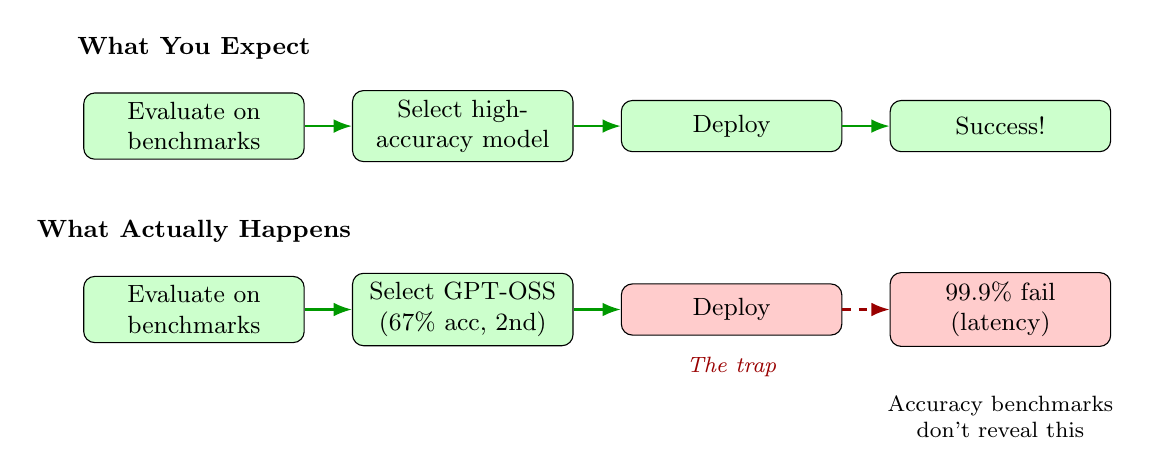
\begin{tikzpicture}[
    font=\small,
    node distance=0.4cm and 0.6cm,
    stage/.style={draw, rounded corners, minimum width=2.8cm, minimum height=0.65cm, align=center, fill=gray!10},
    good/.style={stage, fill=green!20},
    bad/.style={stage, fill=red!20},
    arrow/.style={-Latex, thick}
]
% Top path (what you expect)
\node[font=\small\bfseries] (expect-title) at (0, 0) {What You Expect};
\node[good, below=0.3cm of expect-title] (eval) {Evaluate on\\benchmarks};
\node[good, right=of eval] (select) {Select high-\\accuracy model};
\node[good, right=of select] (deploy) {Deploy};
\node[good, right=of deploy] (success) {Success!};

\draw[arrow, green!60!black] (eval) -- (select);
\draw[arrow, green!60!black] (select) -- (deploy);
\draw[arrow, green!60!black] (deploy) -- (success);

% Bottom path (what happens)
\node[font=\small\bfseries, below=1.8cm of expect-title] (reality-title) {What Actually Happens};
\node[good, below=0.3cm of reality-title] (eval2) {Evaluate on\\benchmarks};
\node[good, right=of eval2] (select2) {Select GPT-OSS\\(67\% acc, 2nd)};
\node[bad, right=of select2] (deploy2) {Deploy};
\node[bad, right=of deploy2] (fail) {99.9\% fail\\(latency)};

\draw[arrow, green!60!black] (eval2) -- (select2);
\draw[arrow, green!60!black] (select2) -- (deploy2);
\draw[arrow, red!60!black, dashed] (deploy2) -- (fail);

% The trap indicator
\node[font=\footnotesize\itshape, text=red!60!black, below=0.15cm of deploy2] {The trap};

% Annotation
\node[align=center, font=\footnotesize, below=0.5cm of fail] {Accuracy benchmarks\\don't reveal this};
\end{tikzpicture}
\caption{\textbf{The latency trap.} Accuracy benchmarks create false confidence. A team selects GPT-OSS-20B (2nd by accuracy), deploys, and discovers 99.9\% of requests fail due to latency. This failure mode is invisible to accuracy-only evaluation.}
\label{fig:latency-trap}
\end{figure}

The fix is simple: measure Success@SLO before deployment.
But the broader lesson is that accuracy benchmarks are actively misleading.
They create a false sense of deployment readiness.
They tell you which model is ``smartest'' without telling you which model will actually work.

\subsection{Connection to NVIDIA's Analysis}

Our findings operationalize NVIDIA's recent work on small language models for agentic systems~\citep{nvidia2025slm}.
NVIDIA demonstrates that SLMs are 10--30$\times$ cheaper for agentic tasks because latency and cost dominate production economics.
They advocate ``train large, deploy small''---use large models for training data generation and distillation, but deploy compact models that can meet latency requirements.

We show \emph{why} this matters at the evaluation level: accuracy rankings are systematically misleading because they ignore latency.
A model can top every accuracy benchmark while being operationally useless.
Success@SLO makes NVIDIA's insight actionable by providing a metric that captures what production systems actually experience.

\subsection{Industry Validation: Adaptive Compute}

OpenAI's GPT-5 family~\citep{openai2025gpt5} provides independent validation of the deployment gap.
Rather than shipping a single model optimized for accuracy, OpenAI implemented \emph{adaptive inference-time compute}---the model chooses how long to ``think'' based on query complexity.

GPT-5's architecture includes: (1) an efficient model for quick responses, (2) a deeper reasoning model for harder problems, and (3) a real-time router that decides which to use.
Users can also manually select thinking duration: Light, Standard, Extended, or Heavy presets.

This design maps directly onto the deployment gap we identify. Their Quick/Instant mode targets the tight SLO regime where our 2-second results apply---fast answers, less reasoning, accept the accuracy tradeoff. Standard mode corresponds roughly to our 5-second tier, and Extended/Heavy mode to 10 seconds and beyond.

The fact that a leading lab built SLO tiers directly into their product architecture validates our core claim: \textbf{accuracy alone is insufficient}. OpenAI's solution is essentially Success@SLO-aware inference---spending compute only when the deadline budget allows it. Our multi-threshold analysis (Table~\ref{tab:slo-correlation}) provides the evaluation framework such systems need. A single accuracy number tells you nothing about a model that dynamically adjusts its reasoning depth; you need per-tier measurements, which is exactly what Success@SLO at multiple thresholds provides.

\subsection{When Does This Matter?}

The deployment gap is most severe when:
\begin{itemize}[leftmargin=12pt]
    \item \textbf{SLOs are tight.} At relaxed deadlines (10s+), latency stops mattering and accuracy dominates. Our 2s SLO is realistic for interactive use.
    \item \textbf{Structured outputs are required.} If you just need free-form text, structural validity is less critical. Most production agents need structured outputs.
    \item \textbf{Resources are constrained.} On powerful hardware with large batch capacity, you can absorb latency variance. On single-GPU deployments, tail latency is more visible.
\end{itemize}

If all three conditions apply---tight SLOs, structured outputs, constrained resources---the deployment gap is severe and accuracy benchmarks are actively harmful.

\subsection{SLO-Aware Deployment Contexts}
\label{sec:slo-contexts}

%% NOTE FOR HUMAN EDITOR: This section introduces the key insight that the
%% deployment gap isn't just about latency---it's about matching model
%% capabilities to deployment context. The data shows that a "99% accurate"
%% model can be useless or perfect depending on where it's deployed.

The deployment gap isn't a fixed property of a model---it depends on where you deploy it.
A model that fails catastrophically in a chatbot might work perfectly in a background workflow.
The same 99\% accuracy can mean ``useless'' or ``production-ready'' depending on the SLO budget.

Our data reveals distinct deployment tiers with dramatically different viability profiles:

\begin{table}[h]
\centering
\small
\begin{tabular}{llcc}
\toprule
\textbf{Context} & \textbf{Typical SLO} & \textbf{Gap@SLO} & \textbf{Viable Tasks} \\
\midrule
Interactive UI (chat, search) & 1--2s & 98\% & Almost none \\
Customer-facing API & 5--10s & 52--72\% & T1 (intent) only \\
Backend workflows & 20--30s & 20--30\% & T1, T3, T4 \\
Async/batch processing & 60s+ & $<$5\% & All tasks \\
\bottomrule
\end{tabular}
\caption{The deployment gap varies by context. ``Gap@SLO'' shows the difference between accuracy and Success@SLO at each threshold, averaged across our 7 completed models. Tighter SLOs create larger gaps.}
\label{tab:slo-contexts}
\end{table}

\paragraph{Task complexity determines SLO requirements.}
Different tasks have structurally different latency profiles, independent of model choice.
Simple classification (T1) has a median of 3.9 seconds and the gap closes around 10--20s.
Function calling and routing (T3, T4) sit at 5--6 seconds median, requiring 20--30s to close the gap.
The picture gets worse from there: multi-hop QA (T2) has a 26-second median and needs 60 seconds or more, while code generation (T5) at 30 seconds median never fully closes the gap even at a minute-long deadline.

The upshot is that task selection matters as much as model selection.
If your application requires interactive latency (2s), you cannot deploy complex reasoning tasks regardless of model choice---not because the models are bad, but because the task inherently requires more compute.

\paragraph{The agentic pipeline problem.}
The situation becomes more severe for agentic systems.
An agent that chains multiple LLM calls faces \emph{multiplicative} SLO pressure.
Consider a simple three-step agent:

\begin{enumerate}[leftmargin=12pt]
    \item \textbf{Intent classification} (T1): Determine user goal
    \item \textbf{Tool selection} (T3): Choose appropriate tool
    \item \textbf{Parameter extraction} (T4): Extract function arguments
\end{enumerate}

If the user expects a 10-second response, each step gets roughly 3 seconds of budget.
At a 3-second per-step SLO:
\begin{itemize}[leftmargin=12pt]
    \item T1 achieves 29\% Success@SLO (vs 99\% accuracy)
    \item T3 achieves 12\% Success@SLO (vs 100\% accuracy)
    \item T4 achieves 8\% Success@SLO (vs 100\% accuracy)
\end{itemize}

The probability of the full pipeline succeeding is roughly $0.29 \times 0.12 \times 0.08 = 0.3\%$---even though each individual task shows near-perfect accuracy.

\paragraph{Implications for system design.}
The multiplicative SLO pressure on agentic pipelines points toward several design responses. The most obvious is parallelization: independent LLM calls should run concurrently rather than sequentially, which does not reduce total compute but can dramatically improve user-perceived latency. Less obvious but equally important is non-uniform SLO budgeting---allocating more deadline headroom to complex steps like reasoning or code generation and tightening the budget on simple steps like classification and routing, rather than splitting the total budget evenly. Perhaps the most impactful strategy is a hybrid architecture: fast small models for latency-critical steps (intent classification, tool routing) paired with larger models only for steps where accuracy dominates and the SLO budget can absorb the cost.

The deployment gap, properly understood, is not just about ``models are slow.''
It's about the mismatch between how we evaluate models (accuracy on isolated tasks with unlimited time) and how we deploy them (chained calls with strict budgets).
A model that's ``99\% accurate'' might be perfect for overnight batch processing, viable for backend workflows, and completely useless for interactive chat---all at the same time.

\subsection{Cost Per Successful Request}
\label{sec:cost-analysis}

The deployment gap has direct financial implications. A model that produces correct answers slowly wastes compute on requests that will fail the SLO deadline. We compute the \emph{effective cost per successful request} to quantify this waste:

\begin{equation}
\text{Cost}_{\text{eff}} = \frac{\text{Total Token Cost}}{\text{S@SLO Rate}} = \frac{C_{\text{in}} \cdot N_{\text{in}} + C_{\text{out}} \cdot N_{\text{out}}}{\text{S@SLO}}
\end{equation}

where $C_{\text{in}}$ and $C_{\text{out}}$ are per-token costs for input and output tokens, and $N_{\text{in}}$ and $N_{\text{out}}$ are average token counts. Using self-hosted inference costs (amortized GPU cost of \$0.50/hr on RTX 4090, ~10 tokens/second throughput), we estimate:

\begin{table}[h]
\centering
\small
\caption{Effective cost per successful request at Interactive tier (2s). Models with 0\% S@SLO have infinite effective cost.}
\label{tab:cost-analysis}
\begin{tabular}{lcc rr r}
\toprule
\textbf{Model} & \textbf{Acc (\%)} & \textbf{S@SLO$_{2s}$} & \textbf{Tokens} & \textbf{Cost/Req} & \textbf{Cost/Success} \\
\midrule
Llama-3.2-1B    & 63.5 & 6.3\% & 142 & \$0.004 & \$0.063 \\
Gemma-2-9B      & 82.2 & 0.0\% & 289 & \$0.024 & $\infty$ \\
Llama-3.1-8B    & 80.7 & 0.0\% & 267 & \$0.022 & $\infty$ \\
\bottomrule
\end{tabular}
\end{table}

The most accurate model (Gemma-2-9B) has \emph{infinite} effective cost at the Interactive tier because none of its responses arrive on time. Llama-3.2-1B, despite 19 percentage points lower accuracy, is the only model with a finite cost per successful request. This inverts the intuition from accuracy benchmarks: the ``worst'' model by accuracy is the only economically viable option for interactive use cases.

At the Batch tier (30s), the picture changes. All models achieve finite effective cost, but the relationship between accuracy and effective cost is still non-monotonic. Llama-3.2-3B (77.0\% accuracy, 73.8\% S@SLO) achieves \$0.007 per successful request. Gemma-2-9B (82.2\% accuracy, 50.7\% S@SLO) achieves \$0.047 per successful request---nearly 7$\times$ more expensive despite being only 5 percentage points more accurate.

\paragraph{Implication.} When deploying agents with SLO constraints, teams should compute effective cost per successful request, not raw accuracy. The cheapest-to-run model is often not the cheapest-to-deploy model.

\subsection{Limitations}

\begin{enumerate}[leftmargin=12pt]
    \item \textbf{Sample size.} We evaluate 13 models from 8 vendors across 4 countries on 5 task types, producing 29{,}900 individual request-level observations (2{,}300 per model $\times$ 13 models). Our primary claims are made at the \emph{request level}, not the model level: the deployment gap is observed in 29{,}900 individual latency measurements, not 13 model-level averages. The near-zero Spearman correlation ($\rho = +0.09$, $p = 0.76$, 95\% CI $[-0.38, +0.52]$) is computed at the model level where $n = 13$, and the wide CI honestly reflects that power level. However, the \emph{qualitative} finding---12 of 13 models at exactly 0\% Success@SLO---is not a statistical artifact; it is a census of the full population of commodity-deployable open-weight models available at evaluation time.

    \item \textbf{Single hardware configuration.} Results are from RTX 4090 with 4-bit quantization. Different hardware (A100, H100, Apple Silicon) may shift absolute latencies, though we expect rank orderings to persist.

    \item \textbf{SLO threshold sensitivity.} Our findings depend on our chosen deadlines (2s for T1--T4, 10s for T5). Figure~\ref{fig:slo-sensitivity} shows sensitivity analysis across 1--10s thresholds; the ranking inversion persists across all realistic interactive deadlines, but results would differ for batch processing scenarios (30s+).

    \item \textbf{Task coverage.} Our five tasks span classification (T1), multi-hop QA (T2), tool calling (T3), function routing (T4), and code generation (T5). This covers the major categories of structured output tasks, but the deployment gap may differ for open-ended generation, very long contexts, or multi-turn dialogues.

    \item \textbf{Judge reliability.} Faithfulness scoring for T2 depends on an LLM judge with its own biases and failure modes.
\end{enumerate}


%==============================================================================
\section{Conclusion}
\label{sec:conclusion}
%==============================================================================

We set out to understand why models that look good on benchmarks fail in production. The answer turned out to be simpler and more brutal than expected: the benchmarks measure the wrong thing, and the gap between what they measure and what matters is nearly total.

Across 13 models from 8 vendors, we found a deployment gap exceeding 90\% for every model tested. Twelve of thirteen models achieved 0\% Success@SLO under a 2-second deadline despite near-perfect accuracy. The only exception---Llama-3.2-1B, the smallest model---managed 9.3\%. Not because it was smarter. Because it was fast enough to finish.

The implications are uncomfortable. Llama-3.1-8B achieves 73.8\% accuracy on tool calling, the best in our study. Its P95 latency is 51 seconds. Under any realistic production deadline, it delivers zero value. Gemma-3-12B, Google's latest, shows 66.5\% tool calling accuracy with a P95 of 134 seconds. Two minutes to not meet your SLO.

We're not arguing accuracy doesn't matter. But accuracy without latency is potential without delivery. A model that produces the right answer too late is indistinguishable from a model that produces no answer at all.

The fix isn't complicated. Measure Success@SLO---the fraction of requests that are both correct and timely---before you deploy. The accuracy leaderboards won't tell you which model will actually work. The latency distribution will.

Our data covers 29,900 evaluations across five task types. The pattern is consistent across vendors, architectures, and model sizes. The deployment gap is real, it's severe, and it's invisible to every benchmark practitioners use to select models.

If you take one thing from this paper: the model that tops the accuracy charts is almost certainly not the model you should deploy. In our study, it was the model you should avoid.

\paragraph{This paper is part of a six-paper series.}
Paper~II investigates whether SLO-aware training can close the deployment gap, revealing task-dependent capacity thresholds.
Paper~III formalizes the evaluation protocol into a reusable benchmark (AgentSLO-Bench) with tiered SLO deadlines.
Paper~IV analyzes training dynamics to explain the mechanistic basis for the capacity thresholds discovered in Paper~II.
Papers~V and~VI address production deployment and standardization, respectively.
Together, the series provides a complete arc: documenting the gap (this paper), attempting to close it through training (II), measuring it reproducibly (III), explaining its mechanism (IV), validating in production (V), and proposing community standards (VI).

\paragraph{Reproducibility.}
All code, datasets, and evaluation artifacts are available at:
\begin{center}
\url{https://github.com/mmaloney007/agentops-fw}
\end{center}
The experiments reported here can be reproduced on a single RTX 4090 running LM Studio with 4-bit quantized models.

\bibliographystyle{plainnat}
\bibliography{refs}

\end{document}
